\documentclass[11pt]{article}
\usepackage[utf8]{inputenc}
\usepackage[margin=1in]{geometry}
\usepackage{graphicx,amsmath,amssymb,booktabs,hyperref,xcolor,subcaption}
\usepackage[numbers,sort&compress]{natbib}
\graphicspath{{../results/}{../results/figures/}}
\hypersetup{colorlinks=true,linkcolor=blue,citecolor=blue,urlcolor=blue}

\title{\textbf{TetraSwarm}: Cooperative Aerial Transport of Tetromino Payloads\\
through Unknown Mazes with Onboard Multi-Drone Mapping}
\author{Kyaw Linn Khant\\\small \texttt{github.com/KyawLinnKhant/TetraSwarm}}
\date{\today}

\begin{document}
\maketitle

\begin{abstract}
We present \textbf{TetraSwarm}, a simulation testbed and integrated pipeline for
cooperative aerial transport of arbitrarily shaped (tetromino) payloads through
cluttered, initially \emph{unknown} environments, using only onboard sensing.
A swarm of quadrotors (i) accepts natural-language formation commands via a
large-language-model commander, (ii) cooperatively lifts a payload whose mass and
geometry are not given a priori, estimating the mass online with an adaptive
controller, (iii) rotates bulky payloads to fit through doorways narrower than the
payload is wide (a piano-mover maneuver), and (iv) explores an unknown braided maze
with a distributed lidar swarm to build a shared occupancy map that the couriers
then plan on---requiring no overhead camera. We describe the perception, planning,
and control components and report qualitative and quantitative results in MuJoCo.
We position the work as an engineering demonstration and testbed that integrates
several active research directions (cooperative manipulation, unknown-payload
adaptive control, informative path planning, and LLM-driven robotics).
\end{abstract}

\section{Introduction}
Cooperative aerial transport---multiple UAVs carrying a single payload---is an
active subfield of aerial manipulation. Most demonstrations assume a known payload
and a known, instrumented environment (e.g.\ motion capture). We instead target the
harder, more realistic setting of an \emph{unknown payload} (mass and geometry) in
an \emph{unknown environment} mapped only by the robots themselves. TetraSwarm
integrates four capabilities into one pipeline: (1) a natural-language commander;
(2) cooperative suction-cup transport with online mass estimation; (3) a turn-to-fit
maneuver for bulky payloads in tight spaces; and (4) distributed multi-drone lidar
mapping of an unknown maze. Figure~\ref{fig:hero} shows the headline scenario.

\begin{figure}[t]\centering
  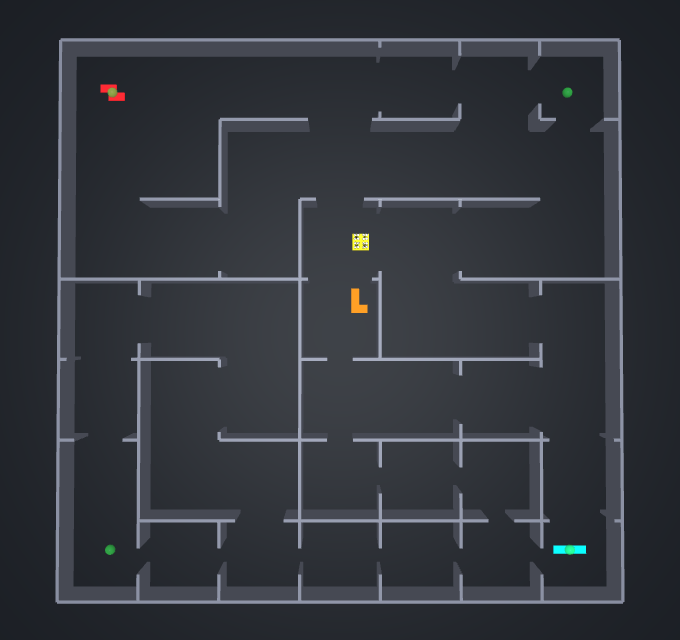
\includegraphics[width=0.62\linewidth]{maze_relay.png}
  \caption{The warehouse maze relay: one swarm delivers four tetromino blocks from
  a central depot to the four maze corners, turning each block to clear the narrow
  doorways, with zero wall contacts.}
  \label{fig:hero}
\end{figure}

\section{Related Work}
We build on cooperative aerial manipulation and slung-load transport, on
model-reference adaptive control for unknown loads, on informative path planning
for autonomous exploration (e.g.\ frontier- and information-gain methods, and the
VIPER line of work), and on recent LLM-as-controller approaches in robotics. Our
contribution is integrative: a reproducible testbed combining these in one system.

\section{System Overview}
The system is organized as perception $\rightarrow$ planning $\rightarrow$ control.
Drones are force-controlled point masses (a PD position controller writing a 6-D
wrench), with a Skydio~X2 visual mesh. Payloads are thin tetromino slabs; suction is
modeled as a rigid \texttt{connect} constraint toggled at contact. Scenes (transport,
navigation, mission, braided maze, relay, scout) are generated programmatically.

\section{Methods}
\subsection{Natural-language formations}
A commander maps an instruction to a validated formation from a registry and
parameters, with an offline keyword fallback. The swarm forms the shape
collision-free by expanding radially from a shrunken copy of the target and
enforcing a hard $1.5$\,m inter-drone spacing (Fig.~\ref{fig:formations}).

\subsection{Cooperative transport and crew sizing}
\texttt{plan\_transport} computes payload mass from tile geometry and density and
the required number of carriers from a per-drone lift capacity with margin. Carriers
run approach, descend, suction-on, lift, and carry phases (Fig.~\ref{fig:sizing}).

\subsection{Online mass estimation (unknown payload)}
With no prior knowledge of the payload, each drone $i$ adds an adaptive vertical
feedforward $w_i$ updated by $w_i \leftarrow w_i + \gamma\,(z^*_i - z_i)\,\Delta t$,
which converges to its share of the load; the total mass is recovered as
$\hat m = \big(\sum_i w_i\big)/g - N m_\text{drone}$ (Fig.~\ref{fig:unknown}).

\subsection{Turn-to-fit}
When the payload is wider than a gap, the carriers yaw the grip formation so the
payload's narrow side leads, completing the rotation before the gap (its diagonal is
wider than either side mid-turn) and slowing forward motion while turning
(Fig.~\ref{fig:turnfit}).

\subsection{Distributed autonomous exploration}
$N$ lidar-equipped drones explore an unknown braided maze with no prior map and no
ground-truth route. Each ray-casts a short-range lidar into a shared log-odds
occupancy grid; the team runs classical decentralized \emph{frontier} exploration
(Yamauchi-style): detect frontiers, cluster them, disperse the drones by angular
sector to different regions, and plan A$^\star$ over the sensed free space behind a
reactive lidar-proximity avoidance layer, so the solid drones finish with zero wall
and zero inter-drone contacts (Fig.~\ref{fig:scout}). We emphasize that this is a
\emph{classical} frontier explorer inspired by the informative-exploration goal of
MarmotLab's VIPER, \emph{not} the learned VIPER policy; substituting a learned
informative-path-planning policy is a direct extension. The couriers then plan
routes and gap widths from the resulting map.

\section{Experiments and Results}
All experiments run in MuJoCo. Formations converge with zero inter-drone collisions
while holding the $1.5$\,m bound (Fig.~\ref{fig:formations}). Online mass estimation
converges to within a few percent across all tetrominoes (Fig.~\ref{fig:unknown}).
The turn-to-fit maneuver delivers through a solid doorway when feasible and is
physically blocked otherwise (Fig.~\ref{fig:turnfit}). Four drones explore the
unknown maze frontier-first with zero wall and zero inter-drone contacts, and the
team maps it faster than a single drone (a modest super-linear-free speedup,
consistent with coordination overhead and shared corridors; Fig.~\ref{fig:scout}).
The maze relay delivers all four blocks with zero wall contacts (Fig.~\ref{fig:hero}).

\begin{figure}[t]\centering
  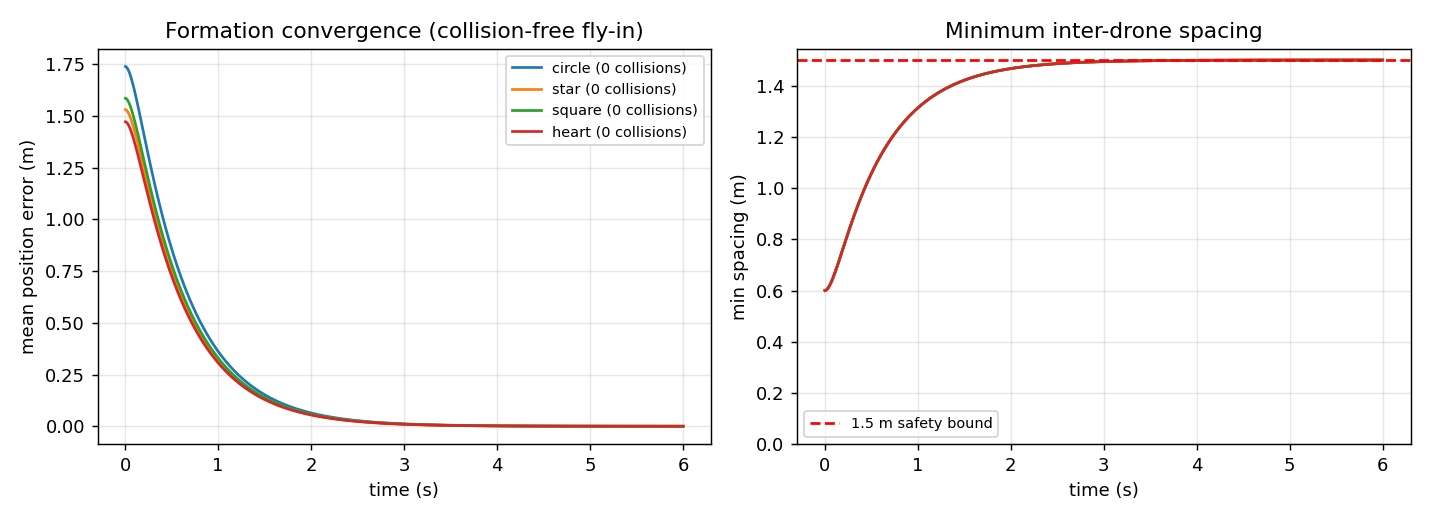
\includegraphics[width=0.85\linewidth]{fig1_formations.png}
  \caption{Formation convergence (collision-free fly-in) and minimum inter-drone
  spacing vs.\ the $1.5$\,m safety bound.}\label{fig:formations}
\end{figure}

\begin{figure}[t]
  \begin{subfigure}{0.5\linewidth}\centering
    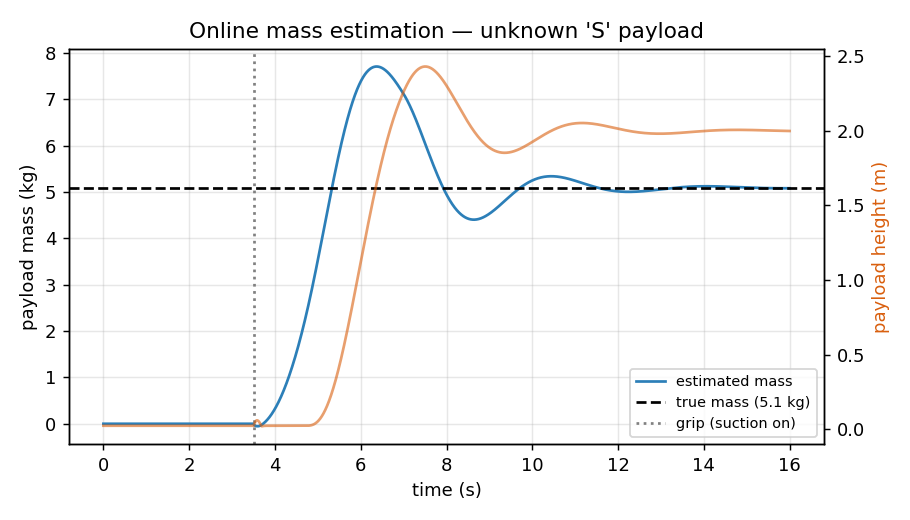
\includegraphics[width=\linewidth]{transport1.png}\caption{}\end{subfigure}
  \begin{subfigure}{0.5\linewidth}\centering
    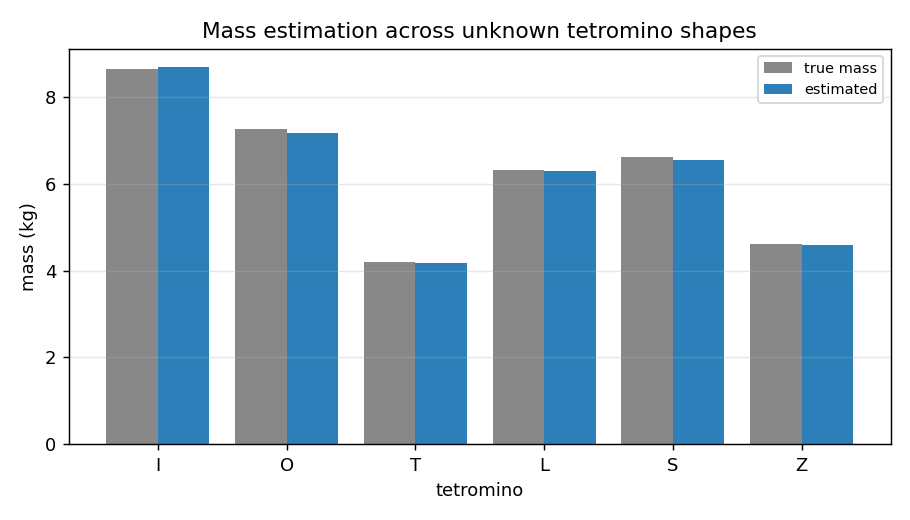
\includegraphics[width=\linewidth]{transport2.png}\caption{}\end{subfigure}
  \caption{Online mass estimation for an unknown payload: (a) the estimate converges
  to the true mass after the grip; (b) estimated vs.\ true mass across all
  tetrominoes.}\label{fig:unknown}
\end{figure}

\begin{figure}[t]\centering
  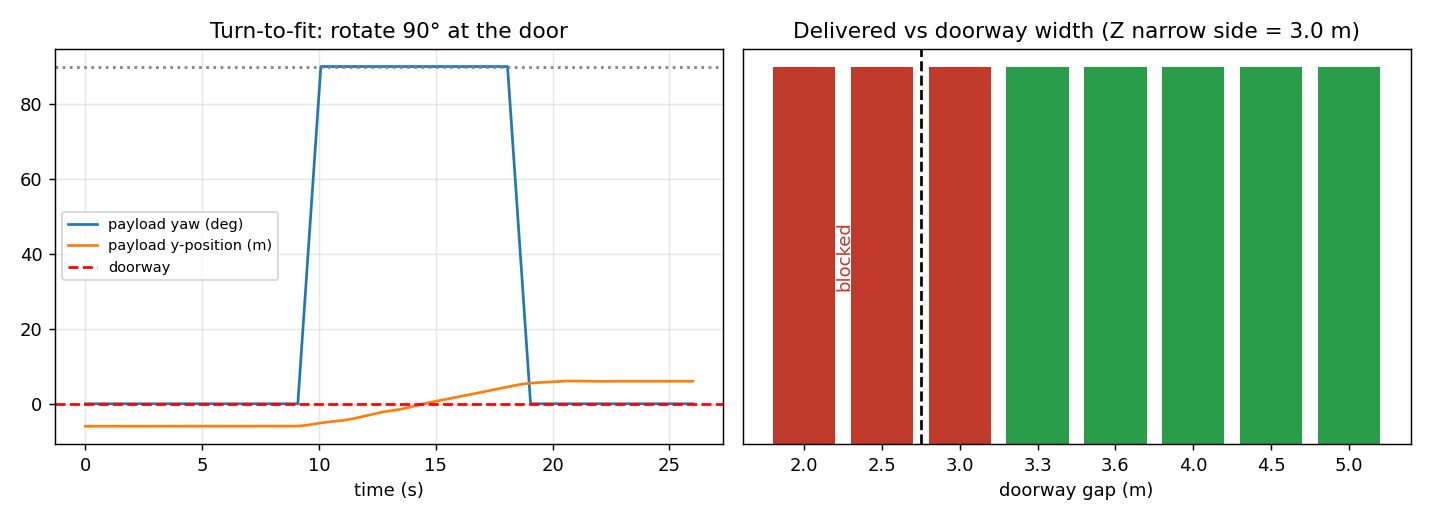
\includegraphics[width=0.85\linewidth]{fig2_turn_to_fit.png}
  \caption{Turn-to-fit: payload yaw vs.\ doorway crossing, and delivery success vs.\
  gap width (blocked when the gap is narrower than the payload's narrow side).}
  \label{fig:turnfit}
\end{figure}

\begin{figure}[t]
  \begin{subfigure}{0.55\linewidth}\centering
    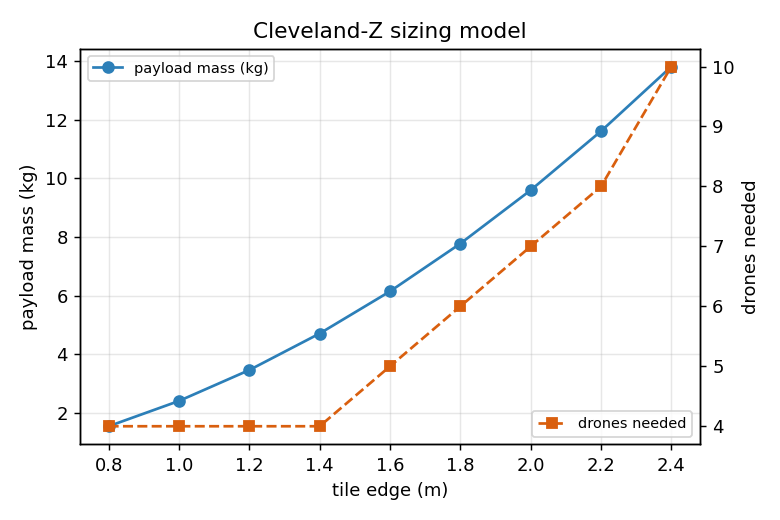
\includegraphics[width=\linewidth]{fig4_sizing.png}\caption{}\end{subfigure}
  \begin{subfigure}{0.43\linewidth}\centering
    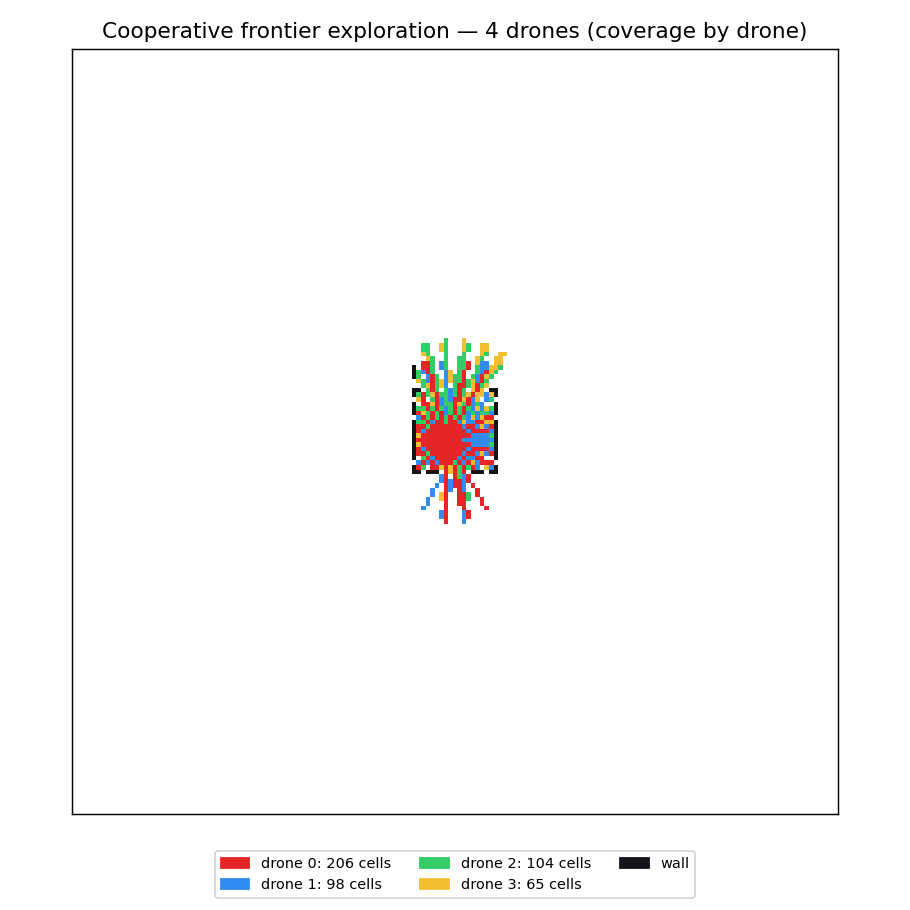
\includegraphics[width=\linewidth]{scout_coverage.png}\caption{}\end{subfigure}
  \caption{(a) Payload-sizing model: mass and required drones vs.\ tile size.
  (b) Distributed VIPER mapping: each drone's mapped region in its own color.}
  \label{fig:scout}
\end{figure}

\section{Limitations}
Suction is an idealized rigid constraint; the carry/relay drones are kinematically
driven for clean visualization rather than fully dynamically simulated; the X2 model
is visual (no rotor-level thrust); and the VIPER scout is a heuristic corridor
explorer rather than a learned informative-path-planning policy. These are the
natural next steps toward a quantitatively benchmarked study.

\section{Conclusion}
TetraSwarm integrates LLM commanding, cooperative unknown-payload transport,
turn-to-fit maneuvering, and distributed onboard mapping into one reproducible
MuJoCo testbed for cooperative transport in unknown environments without external
infrastructure.

\bibliographystyle{plainnat}
\bibliography{refs}
\end{document}
